\section{Rendering}
\label{sec:rendering}

In conjuction with creating our own GUI library, we've also created objects 
that handle the rendering of entities and UIComponents. This class is called 
the RenderObject, which is also a templated class so that we can reuse it 
if and when we decide to switch over to OpenGL rendering.

The Rendering class and its derived classes can be seen in 
\cref{fig:renderobject-inherit}.

\begin{figure}[!htb]
\centering
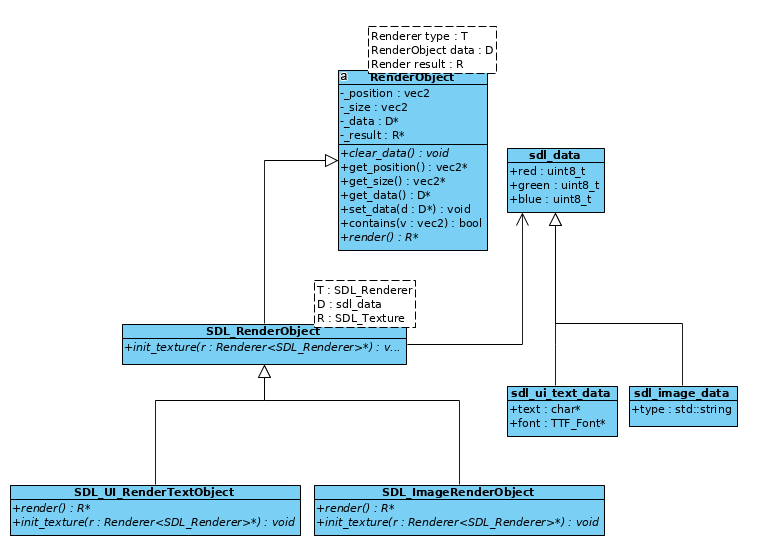
\includegraphics[scale=0.55]{res/renderobject-inherit.png}
\caption{RenderObject and derived classes}\label{fig:renderobject-inherit}
\end{figure}

\newpage
\subsection{Objects as a proxy}
\label{sec:rendering-proxy}

Objects that need to be rendered to the screen act as a proxy for the 
RenderObject. The only thing those objects need to do to be rendered can be 
seen in \cref{lst:rendering}. As you can see, the objects only need to return 
the result of its own RenderObject. Objects that need custom rendering logic 
can have a rendering object that derives from the SDL\_RenderObject class seen 
in \cref{fig:renderobject-inherit}.
\\
\begin{lstlisting}[caption={Rendering proxy.},label={lst:rendering}]
void BaseEntity::render(SDLRenderer *renderer) {
    return representation->render(renderer);
}
\end{lstlisting}

When a RenderObject renders itself, it sends the texture it created to the 
SDLRenderer class to draw it on a back buffer. After the rendering loop is 
completed, the back buffer is drawn to the screen using the 
\lstinline{renderer->draw_to_back_buffer(SDL_Texture *, SDL_Rect *)} 
method shown in \cref{lst:drawtobackbuffer}.
\\

\begin{lstlisting}[caption={Drawing to the back buffer.},
label={lst:drawtobackbuffer}]
void SDLRenderer::draw_to_back_buffer(SDL_Texture *t, SDL_Rect *r) {
    SDL_SetRenderTarget(engine, _back_buffer);
    // Blend the textures
    SDL_SetTextureBlendMode(_back_buffer, SDL_BLENDMODE_BLEND);
    SDL_SetTextureBlendMode(t, SDL_BLENDMODE_BLEND);
    if (SDL_RenderCopy(engine, t, NULL, r) < 0) {
        std::cerr << SDL_GetError() << std::endl;
    }
    SDL_SetRenderTarget(engine, NULL);
}
\end{lstlisting}

\newpage
\subsection{UIComponent Rendering}
\label{sec:rendering-ui}

The uicomponents need a way of rendering their child components after 
rendering themselves. You can think of the relation between child components 
and their parent as a tree in which we first render the parent and then its 
children. The code for rendering a component and its children can be 
seen in \cref{lst:uicomponent-rendering}.
\\
\begin{lstlisting}[caption={UIComponent rendering.},
label={lst:uicomponent-rendering}]
void SDL_UIComponent::render(SDLRenderer *renderer, float delta) {
    representation->render(renderer);

    for (int i = 0; i < this->children.size(); i++) {
        children[i]->render(renderer, delta);
    }
}
\end{lstlisting}

